\documentclass[border=2pt]{standalone}
\usepackage{pgfplots}
\usepackage{xcolor}

\pgfplotsset{compat=1.18}

\definecolor{Garnet}{HTML}{73000A}
\definecolor{Gray10}{gray}{0.10}
\definecolor{Gray30}{gray}{0.30}
\definecolor{Gray50}{gray}{0.50}
\definecolor{Gray70}{gray}{0.70}
\definecolor{Gray90}{gray}{0.90}

\pgfplotsset{
  every axis/.style={
    axis line style={draw=black, line width=0.6pt},
    tick style={draw=black, line width=0.6pt},
    tick label style={font=\footnotesize\color{black}},
    label style={font=\small\color{black}},
    grid=both,
    grid style={draw=Gray90, line width=0.3pt},
    legend style={
      draw=none,
      font=\footnotesize\color{black},
      fill=white,
      at={(0.95,0.05)},
      anchor=south east,
    },
  },
  linestyle/.style={
    line width=0.8pt,
    mark=none,
  },
}
\begin{document}


% SO-DETR mAP50
\begin{figure}[h]
\centering
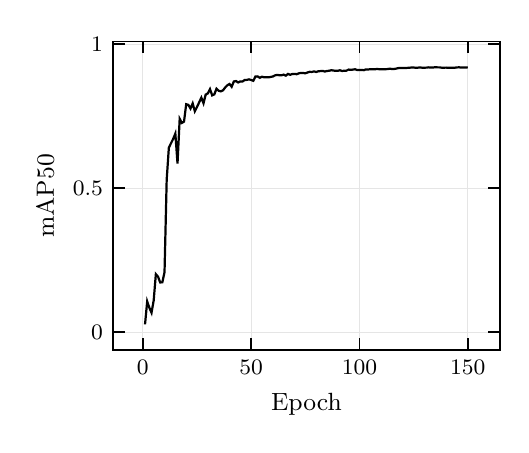
\begin{tikzpicture}
\begin{axis}[
  xlabel={Epoch},
  ylabel={mAP50},
  width=6.5cm,
  height=5.5cm,
]
\addplot[linestyle, color=black] coordinates {
  (1,0.026740)
  (2,0.106420)
  (3,0.084290)
  (4,0.067080)
  (5,0.109940)
  (6,0.201020)
  (7,0.192390)
  (8,0.172030)
  (9,0.172980)
  (10,0.207680)
  (11,0.528770)
  (12,0.640300)
  (13,0.655710)
  (14,0.670740)
  (15,0.689290)
  (16,0.585370)
  (17,0.740370)
  (18,0.726050)
  (19,0.730630)
  (20,0.790970)
  (21,0.788870)
  (22,0.775960)
  (23,0.793850)
  (24,0.766520)
  (25,0.781420)
  (26,0.797570)
  (27,0.813840)
  (28,0.794350)
  (29,0.824450)
  (30,0.828700)
  (31,0.843550)
  (32,0.821620)
  (33,0.825300)
  (34,0.844880)
  (35,0.837670)
  (36,0.835720)
  (37,0.839320)
  (38,0.849020)
  (39,0.856800)
  (40,0.861210)
  (41,0.851650)
  (42,0.869950)
  (43,0.871510)
  (44,0.866540)
  (45,0.870300)
  (46,0.869830)
  (47,0.875110)
  (48,0.875510)
  (49,0.877280)
  (50,0.875090)
  (51,0.872200)
  (52,0.887350)
  (53,0.887730)
  (54,0.882750)
  (55,0.886530)
  (56,0.884390)
  (57,0.884850)
  (58,0.884220)
  (59,0.885800)
  (60,0.887250)
  (61,0.891200)
  (62,0.892720)
  (63,0.891700)
  (64,0.891540)
  (65,0.893670)
  (66,0.890180)
  (67,0.896310)
  (68,0.893180)
  (69,0.895980)
  (70,0.896410)
  (71,0.895150)
  (72,0.898260)
  (73,0.899650)
  (74,0.899480)
  (75,0.898390)
  (76,0.901140)
  (77,0.903580)
  (78,0.903040)
  (79,0.904960)
  (80,0.903020)
  (81,0.905520)
  (82,0.906000)
  (83,0.906760)
  (84,0.904460)
  (85,0.906420)
  (86,0.907240)
  (87,0.909010)
  (88,0.908000)
  (89,0.906890)
  (90,0.907000)
  (91,0.908970)
  (92,0.906450)
  (93,0.907270)
  (94,0.907590)
  (95,0.911350)
  (96,0.910390)
  (97,0.911270)
  (98,0.912420)
  (99,0.909420)
  (100,0.909940)
  (101,0.909900)
  (102,0.909280)
  (103,0.911820)
  (104,0.911520)
  (105,0.912670)
  (106,0.912820)
  (107,0.912160)
  (108,0.913470)
  (109,0.912690)
  (110,0.912180)
  (111,0.912300)
  (112,0.912660)
  (113,0.913050)
  (114,0.914410)
  (115,0.913370)
  (116,0.913340)
  (117,0.914780)
  (118,0.916450)
  (119,0.916470)
  (120,0.916440)
  (121,0.916830)
  (122,0.917160)
  (123,0.917600)
  (124,0.918400)
  (125,0.918290)
  (126,0.917750)
  (127,0.918000)
  (128,0.918610)
  (129,0.917770)
  (130,0.917870)
  (131,0.918140)
  (132,0.919070)
  (133,0.918110)
  (134,0.918590)
  (135,0.919440)
  (136,0.918980)
  (137,0.918950)
  (138,0.917810)
  (139,0.917880)
  (140,0.918140)
  (141,0.917390)
  (142,0.917920)
  (143,0.918000)
  (144,0.917810)
  (145,0.918790)
  (146,0.919180)
  (147,0.918200)
  (148,0.918530)
  (149,0.918510)
  (150,0.918110)
};
\end{axis}
\end{tikzpicture}
\end{figure}

% SO-DETR mAP50-95
\begin{figure}[h]
\centering
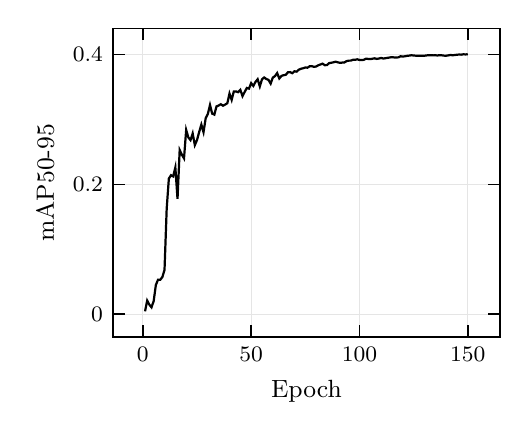
\begin{tikzpicture}
\begin{axis}[
  xlabel={Epoch},
  ylabel={mAP50-95},
  width=6.5cm,
  height=5.5cm,
]
\addplot[linestyle, color=black] coordinates {
  (1,0.004610)
  (2,0.021170)
  (3,0.014810)
  (4,0.010760)
  (5,0.020540)
  (6,0.045180)
  (7,0.053260)
  (8,0.053080)
  (9,0.057320)
  (10,0.068400)
  (11,0.162640)
  (12,0.209140)
  (13,0.214330)
  (14,0.212470)
  (15,0.226230)
  (16,0.177810)
  (17,0.253090)
  (18,0.245930)
  (19,0.240250)
  (20,0.284060)
  (21,0.272480)
  (22,0.268390)
  (23,0.278620)
  (24,0.260690)
  (25,0.268500)
  (26,0.280880)
  (27,0.292280)
  (28,0.280590)
  (29,0.301950)
  (30,0.308760)
  (31,0.322430)
  (32,0.309190)
  (33,0.307650)
  (34,0.320390)
  (35,0.321700)
  (36,0.323650)
  (37,0.321420)
  (38,0.323150)
  (39,0.325160)
  (40,0.340080)
  (41,0.330310)
  (42,0.343410)
  (43,0.343420)
  (44,0.342190)
  (45,0.345810)
  (46,0.336170)
  (47,0.342560)
  (48,0.348710)
  (49,0.347730)
  (50,0.356130)
  (51,0.351840)
  (52,0.358090)
  (53,0.362140)
  (54,0.351070)
  (55,0.362030)
  (56,0.364850)
  (57,0.362520)
  (58,0.361130)
  (59,0.355400)
  (60,0.364730)
  (61,0.366940)
  (62,0.371690)
  (63,0.363360)
  (64,0.367310)
  (65,0.368360)
  (66,0.369000)
  (67,0.372990)
  (68,0.373130)
  (69,0.371490)
  (70,0.374430)
  (71,0.373840)
  (72,0.376850)
  (73,0.378290)
  (74,0.379090)
  (75,0.380190)
  (76,0.379960)
  (77,0.382080)
  (78,0.382360)
  (79,0.381240)
  (80,0.381800)
  (81,0.383690)
  (82,0.384930)
  (83,0.386130)
  (84,0.383780)
  (85,0.384000)
  (86,0.386970)
  (87,0.387530)
  (88,0.388250)
  (89,0.389190)
  (90,0.388220)
  (91,0.387400)
  (92,0.387790)
  (93,0.387910)
  (94,0.390000)
  (95,0.390770)
  (96,0.390870)
  (97,0.392080)
  (98,0.392110)
  (99,0.392900)
  (100,0.391820)
  (101,0.391740)
  (102,0.392020)
  (103,0.393860)
  (104,0.393420)
  (105,0.393130)
  (106,0.393770)
  (107,0.394330)
  (108,0.393480)
  (109,0.394060)
  (110,0.394910)
  (111,0.394050)
  (112,0.394540)
  (113,0.395140)
  (114,0.395690)
  (115,0.396160)
  (116,0.395770)
  (117,0.395620)
  (118,0.395900)
  (119,0.397580)
  (120,0.397010)
  (121,0.397530)
  (122,0.398240)
  (123,0.398550)
  (124,0.399120)
  (125,0.398720)
  (126,0.398440)
  (127,0.398260)
  (128,0.398450)
  (129,0.398240)
  (130,0.398380)
  (131,0.398870)
  (132,0.399120)
  (133,0.399070)
  (134,0.398920)
  (135,0.399130)
  (136,0.398730)
  (137,0.399280)
  (138,0.399010)
  (139,0.398530)
  (140,0.398400)
  (141,0.398860)
  (142,0.399520)
  (143,0.399120)
  (144,0.399480)
  (145,0.399900)
  (146,0.400200)
  (147,0.400000)
  (148,0.400620)
  (149,0.400320)
  (150,0.400700)
};
\end{axis}
\end{tikzpicture}
\end{figure}



\end{document}
